\documentclass[]{article}

\usepackage{array}
\usepackage{mdwmath}
\usepackage{mdwtab}
\usepackage{eqparbox}
%\usepackage[caption=false,font=footnotesize]{subfig}

\usepackage{caption}
\usepackage{subcaption}

\usepackage{fixltx2e}
\usepackage{stfloats}
\usepackage{url}
\usepackage{authblk}

\usepackage[utf8]{inputenc}
\usepackage{times}
\usepackage{amssymb,amsfonts,amsmath,amscd}
\usepackage[pdftex]{hyperref}
\usepackage[pdftex]{graphicx}
\usepackage{fnpos}
\usepackage{multicol}
\usepackage{multirow}
\usepackage{wasysym}
\usepackage{enumerate}
\usepackage{enumitem}
\usepackage{tikz}
\usetikzlibrary{calc}
\usepackage{pgfplots}
\usepackage{listings}
\usepackage{framed}
\usepackage{courier}
\setcounter{MaxMatrixCols}{20}
\usepackage{epsfig}
\usepackage{comment}
\usepackage[space]{cite}
\usepackage{titling}

\bibliographystyle{plain}
\DeclareGraphicsExtensions{.pdf,.jpeg,.png,.eps}
\graphicspath{{figures/}}

% General page formatting
\vfuzz2pt
\hfuzz2pt
\addtolength{\hoffset}{-0.8in} \addtolength{\voffset}{-0.75in}
\setlength{\textwidth}{6.7in} \setlength{\textheight}{8.25in}
\setlength{\headheight}{0.6in}
\setlength{\headsep}{0.55in}
\setlength{\footskip}{40pt}
\setlength{\fboxsep}{12pt}
\setlength{\parskip}{3pt}
\makeFNbottom \makeFNbelow
\setcounter{MaxMatrixCols}{20}

% Math definitions
\newcommand{\norm}[1]{\left\Vert#1\right\Vert}
\newcommand{\abs}[1]{\left\vert#1\right\vert}
\newcommand{\set}[1]{\left\{#1\right\}}
\newcommand{\To}{\longrightarrow}
\newcommand{\Ker}{\textup{Ker}}
\newcommand{\Img}{\textup{Img}}
\newcommand{\diag}{\textup{diag}}
\newcommand{\circulant}{\textup{circ}}
\newcommand{\bcf}{\;\mbox{\boldmath ${\cal F}$\unboldmath}}
\def\Vec#1{\!\!\hbox{$#1$\kern-0.38em\lower0.85em\hbox{$\vec{}\,$}}\,}%
\newcommand{\bbm}{\begin{bmatrix}}
\newcommand{\ebm}{\end{bmatrix}}
\newcommand{\mbf}[1]{\mathbf{#1}}
\newcommand{\mbs}[1]{{\boldsymbol{#1}}}
\newcommand{\mbb}[1]{{\mathbb{#1}}}
\newcommand{\mc}[1]{\mathcal{#1}}
\newcommand{\argmin}{\operatornamewithlimits{argmin}}
\newcommand{\argmax}{\operatornamewithlimits{argmax}}
\newcommand{\expect}{\operatornamewithlimits{\mbb{E}}}

\setlength{\droptitle}{-10em}   % This is your set screw
\begin{document}

\title{Robostats Project Proposal \\ Sparse Planning Graphs for Information \\ Driven Simultaneous Localization and Mapping}
\author{Vishnu Desaraju}
\author{John Yao}
\author{Erik Nelson}
\affil{The Robotics Institute, Carnegie Mellon University\\ \{rajeswar, johnyao, enelson\}@cmu.edu}

\maketitle

\section{Motivation}

\section{Problem Definition}

\begin{figure}[t]
\centering
\begin{subfigure}[b]{0.3\textwidth}
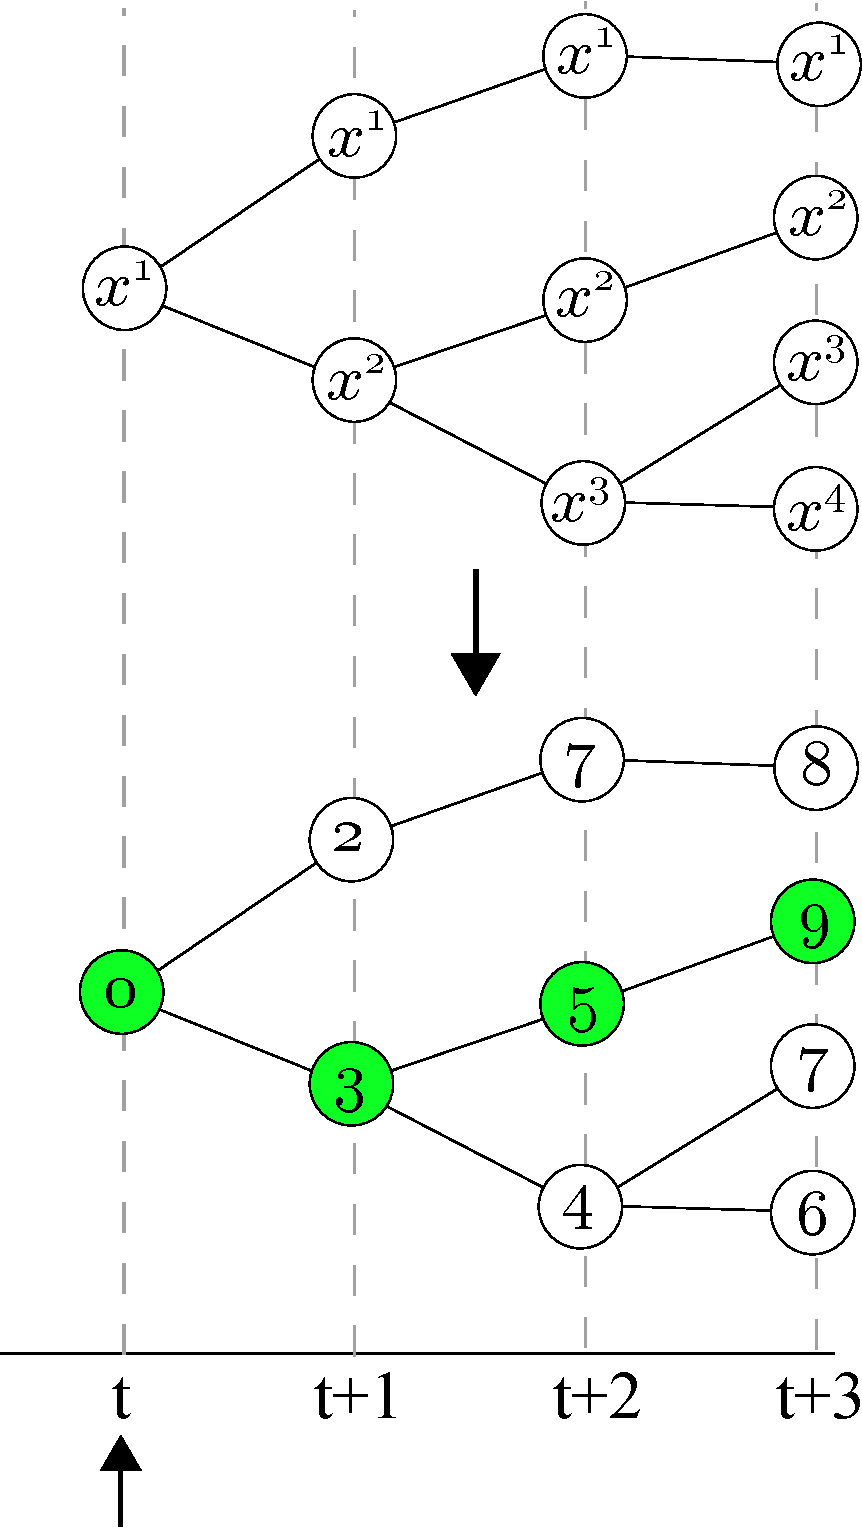
\includegraphics[height=3in]{plan_at_t0}
\caption{A gull}
\label{fig:plan_at_t0}
\end{subfigure}
\hspace{1in}
\begin{subfigure}[b]{0.3\textwidth}
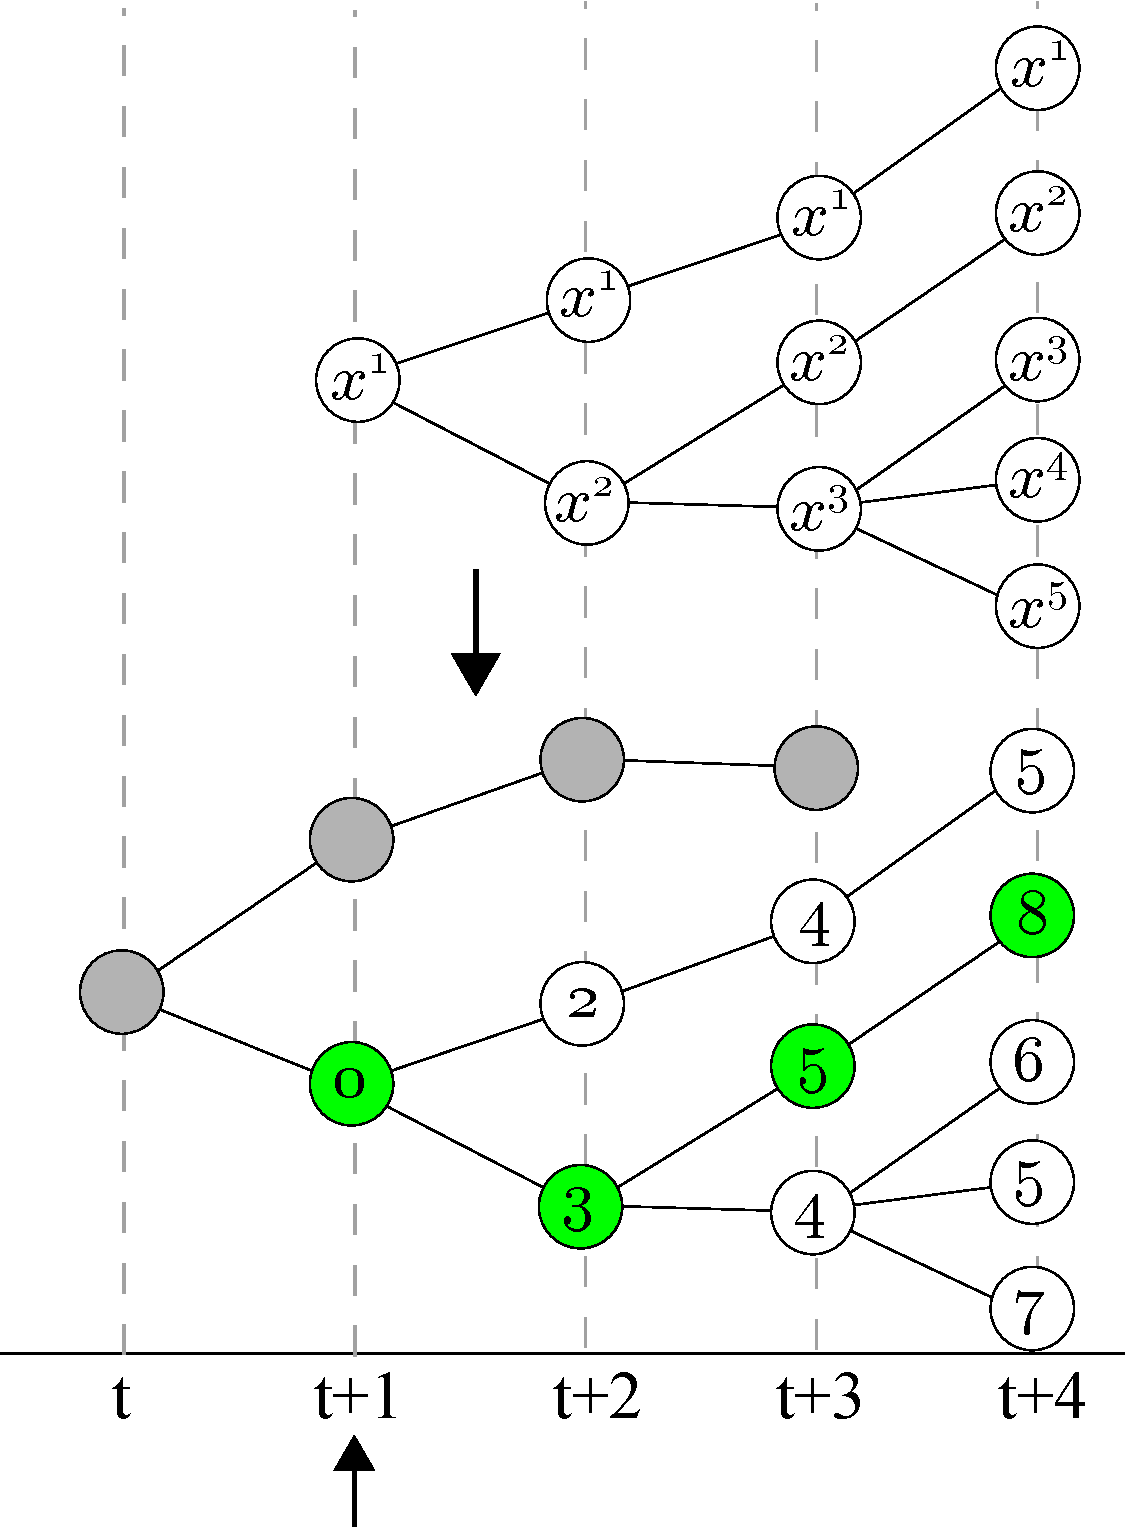
\includegraphics[height=3in]{plan_at_t1}
\caption{A mouse}
\label{fig:plan_at_t1}
\end{subfigure}%

\end{figure}


Our goal is to enable receding horizon planning for active SLAM in a computationally tractable formulation. The active SLAM exploration problem can be framed as determining the control actions which guide a robot to a state that maximizes mutual information between its current and future maps. We model the environment as an occupancy grid map, and represent the map as a conglomeration of cells: $m = \{m^{i}\}_{i=1}^{N}$. The probability that an individual cell is occupied at $t$ is given by $p\left(m^{i} \ \vert \ x_{1:t}, z_{1:t}\right)$, where $x_{1:t}$ denotes the history of states of the vehicle, and $z_{1:t}$ denotes the history of range observations accumulated by the vehicle. Additionally we assume that cell occupancies  are independent of one another: $p\left(m \ \vert \ x_{1:t}, z_{1:t}\right) = \prod_{i} p\left(m^{i} \ \vert \ x_{1:t}, z_{1:t}\right)$. For notational simplicity we write the map conditioned on random variables $x_{1:t}$ and $z_{1:t}$ as $p\left(m_{t}\right) \equiv p\left(m \ \vert \ x_{1:t}, z_{1:t}\right)$.

The optimal plan over a one step horizon will guide the robot to a state, $x_{t+1}^{*}$, in which the mutual information between $m_{t}$ and $m_{t+1}$ is maximized.

\begin{align} \begin{split}
    x_{t+1}^{*}
    &=
    \argmax_{x_{t+1}}
    \
    \text{IG}\left[
        m_{t}
        ;
        m_{t+1}
    \right]
    \\
    &=
    \argmax_{x_{t+1}}
    \
    \text{H}\left[
        m_{t}
    \right]
    -
    \expect_{z_{t+1}}\left[
        \text{H}\left[
            m_{t+1}
        \right]
    \right]
    \\
    &=
    \argmin_{x_{t+1}}
    \
    \expect_{z_{t+1}}\left[
        \text{H}\left[
            m_{t+1}
        \right]
    \right]
\end{split} \end{align}

The term $\text{H}\left[m_{t}\right]$ is independent of the future state $x_{t+1}$, so the information gain is maximized when $x_{t+1}$ minimizes the expected entropy of the updated map. The independence between cell occupancies allows us to write the future entropy of the map as a sum of future entropies of individual grid cells:

\begin{align} \begin{split}
    \text{H}\left[
        m_{t+1}
    \right]
    &=
    \sum_{i=1}^{N}
    \text{H}\left[
        m_{t+1}^{i}
        \ \vert \
        m_{t+1}^{i-1}
        , \
        \dots
        \ ,
        m_{t+1}^{1}
    \right]
    \\
    &=
    \sum_{i=1}^{N}
    \text{H}\left[
        m_{t+1}^{i}
    \right]
\end{split} \end{align}

The expectation to minimize is therefore

\begin{align} \begin{split}
    \expect_{z_{t+1}}\left[
        \text{H}\left[
            m_{t+1}
        \right]
    \right]
    &=
    \int
    p\left(
        z_{t+1}
    \right)
    \sum_{i=1}^{N}
    \text{H}\left[
        m_{t+1}^{i}
    \right]
    dz_{t+1}
    \\
    &=
    -\expect_{z_{t+1}}\left[
        \sum_{i=1}^{N}
        \log p\left(
            m_{t+1}^{i}
        \right)
    \right]
\end{split} \end{align}

\section{Metrics for Success}

In order to reflect on our final result, we have defined the following success metrics:

\begin{enumerate}
  \item Development of a recursive formulation for efficiently solving expected mutual information over several time steps.
  \item Expected mutual information is similar to ground truth mutual information (evaluated in simulation).
  \item Implementation on a quadrotor system demonstrates that the quadrotor navigates towards unexplored areas.
  \item Implementation is real-time for a 2-step horizon, at minimum.
\end{enumerate}

\section{Required Resources}

\subsection*{Software}
\begin{itemize}[noitemsep,topsep=0pt]
\item C++ / ROS Implementation of a laser-based SLAM pipeline (for collecting datasets)
\item Eigen / Armadillo math libraries
\item MATLAB for idea prototyping and plotting
\end{itemize}

\subsection*{Hardware}
\begin{itemize}[noitemsep,topsep=0pt]
\item Vicon motion capture system (for ground truth in datasets)
\item Hokuyo UTM-30LX laser scanner
\end{itemize}

\section{Timeline}

\begin{table}[!ht]
  \centering
  \begin{tabular}{|l|p{13.5 cm} | } \hline
    \textbf{Date} & \textbf{Task / \textcolor{red}{Deliverable}} \\ \hline
            \textcolor{red}{Oct 2} & \textcolor{red}{Written proposal} \\ \hline
            Oct 3 - 8 & Derive bounds on the convergence of the predicted information gain to the actual information gain \\ \hline
            \textcolor{red}{Oct 9} & \textcolor{red}{Initial presentation} \\ \hline
            Oct 9 - 14 & Simulate using a toy example (state-only, no map) \\ \hline
            Oct 15 - 21 & Transition to testing on a quadrotor-mounted laser scanner \\ \hline
            Oct 22 - 29 & Do something ... \\ \hline
            Oct 30 - Nov 5 & Prepare midterm report \\ \hline
            \textcolor{red}{Nov 6} & \textcolor{red}{Midterm report} \\ \hline
            Nov 7 - Nov 13 & Do something ... \\ \hline
            Nov 14 - Nov 19 & Prepare 3 / 4 report \\ \hline
           \textcolor{red}{Nov 20} & \textcolor{red}{3 / 4 report} \\ \hline
             Nov 21 - Nov 27 & Die from overwork ... \\ \hline
            Nov 28 - Dec 3 & Prepare final presentation and video \\ \hline
            \textcolor{red}{Dec 4} & \textcolor{red}{Final presentation} \\ \hline
            Dec 5 - Dec 9 & Prepare final report \\ \hline
           \textcolor{red}{Dec 10} & \textcolor{red}{Final report} \\ \hline
  \end{tabular}
  \caption{Robostats project timeline}
  \label{tab:timeline}
\end{table}



\bibliography{refs}

\end{document}


% Cover in the proposal:
% ==================================================================================
% What are some impacts of this research?
% What is novel about the approach you are taking?
% How do learning and/or probabilistic inference techniques play a key role?
% What is your metric for success?
% What are key technical issues you will have to confront? Any other big challenges?
% What software or data sets will you use?
% What is your timeline? Include specic targets for the progress report.
% ==================================================================================
